%%%%%%%%%%%%%%%%%%%%%%%%%%%%%%%%%%%%%%%%%%%%%%%%%%%%%%%%%%%%%%%%%%%%%%%%%%%%%%%%%%%%%%%%%%%%%%%%%
%
% Document:     Data Management  product tree
%
%%%%%%%%%%%%%%%%%%%%%%%%%%%%%%%%%%%%%%%%%%%%%%%%%%%%%%%%%%%%%%%%%%%%%%%%%%%%%%
\documentclass{article}
\usepackage{times,layouts}
\usepackage{tikz,hyperref,amsmath}
\usetikzlibrary{positioning,arrows,shapes,decorations.shapes,shapes.arrows}
\usetikzlibrary{backgrounds,calc}
\usepackage[paperwidth=411.99999999999994pt,paperheight=301pt,
left=-2mm,top=3mm,bottom=0mm,right=0mm,
noheadfoot,marginparwidth=0pt,includemp=false,
textwidth=30cm,textheight=50mm]{geometry}
\newcommand\showpage{%
\setlayoutscale{0.5}\setlabelfont{\tiny}\printheadingsfalse\printparametersfalse
\currentpage\pagedesign}
\hypersetup{pdftitle={Data Management products }, pdfsubject={Diagram illustrating the
                products in LSST Data Management }, pdfauthor={Extracted from MagicDraw}}
\tikzstyle{tbox}=[rectangle,text centered, text width=30mm]
\tikzstyle{wbbox}=[rectangle, rounded corners=3pt, draw=black, top color=blue!50!white,
                    bottom color=white, very thick, minimum height=40pt, inner sep=2pt,
                    text centered, text width=30mm]
\tikzstyle{pbox}=[rectangle, rounded corners=3pt, draw=black, top
 color=yellow!50!white, bottom color=white, very thick,
 minimum height=36pt, inner sep=3pt, text centered, text width=35mm]
\tikzstyle{pline}=[-, thick]
\begin{document}
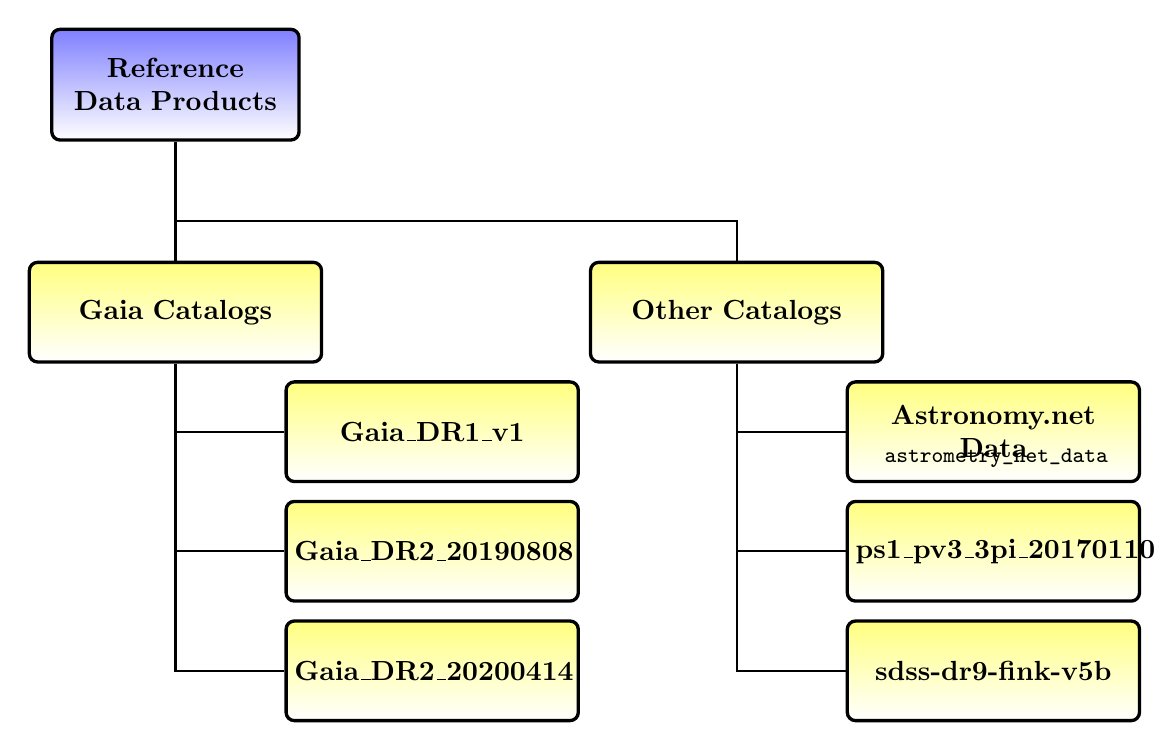
\begin{tikzpicture}[node distance=0mm]


\node (GAIAD) [pbox, 
] {\textbf{Gaia Catalogs
} };\node [below right] at (GAIAD.north west) {\footnotesize \color{blue}} ;

\node (GDR1v1) [pbox,below right=6pt and -14pt of GAIAD] {\textbf{Gaia\_DR1\_v1
} };\node [below right] at (GDR1v1.north west) {\footnotesize \color{blue}} ;

 \draw[pline] (GAIAD.south) -| ++(0,0) |- (GDR1v1.west); 
\node (GDR2198) [pbox,below=6pt of GDR1v1] {\textbf{Gaia\_DR2\_20190808
} };\node [below right] at (GDR2198.north west) {\footnotesize \color{blue}} ;

 \draw[pline] (GAIAD.south) -| ++(0,0) |- (GDR2198.west); 
\node (GDR2204) [pbox,below=6pt of GDR2198] {\textbf{Gaia\_DR2\_20200414
} };\node [below right] at (GDR2204.north west) {\footnotesize \color{blue}} ;

 \draw[pline] (GAIAD.south) -| ++(0,0) |- (GDR2204.west); 
\node (ODATA) [pbox, 
right=96pt of GAIAD] {\textbf{Other Catalogs
} };\node [below right] at (ODATA.north west) {\footnotesize \color{blue}} ;

\node (AND) [pbox,below right=6pt and -14pt of ODATA] {\textbf{Astronomy.net Data
} };\node [below right] at (AND.north west) {\footnotesize \color{blue}} ;
\node (ANDpkg) [tbox,below=3mm of AND.north] {{\footnotesize \color{black} \begin{verbatim} astrometry_net_data \end{verbatim} }  };

 \draw[pline] (ODATA.south) -| ++(0,0) |- (AND.west); 
\node (PS1PV3) [pbox,below=6pt of AND] {\textbf{ps1\_pv3\_3pi\_20170110
} };\node [below right] at (PS1PV3.north west) {\footnotesize \color{blue}} ;

 \draw[pline] (ODATA.south) -| ++(0,0) |- (PS1PV3.west); 
\node (SDSSDR9v5b) [pbox,below=6pt of PS1PV3] {\textbf{sdss-dr9-fink-v5b
} };\node [below right] at (SDSSDR9v5b.north west) {\footnotesize \color{blue}} ;

 \draw[pline] (ODATA.south) -| ++(0,0) |- (SDSSDR9v5b.west); 
\node (REFD) [wbbox, above=43pt of GAIAD]{\textbf{Reference Data Products}};
 \draw[pline]   (GAIAD.north) -- ++(0.0,0.5) -| (REFD.south) ; 
 \draw[pline]   (ODATA.north) -- ++(0.0,0.5) -| (REFD.south) ; 

\end{tikzpicture}
\end{document}
